\documentclass{article}
\usepackage[utf8]{inputenc}

\title{SynthStackSearch}
\author{Amir Salimi}
\date{December 2019}

\usepackage{float}
\usepackage{natbib}
\usepackage{graphicx}
\usepackage{todonotes}
\usepackage{etoolbox}

\begin{document}
\maketitle

\section{Introduction}
\subsection{Purpose of this document}
The purpose of this document is to give a summary of what has been done for this project so far and what needs to be done in the future. Also, to facilitate setting of milestones for what should be done before the up-coming NIME paper deadline; taking into account Dr.Hindle's purported exile on Janurary 1st. The bulk of the paper should be done within the next 2-3 weeks and the focus should be on improvements from then on. 
\subsection{Purpose of project}
The purpose of this project is to synthetically generate high-quality and novel one-shot drum samples of various categories. Each category of drum being defined by example; using numerous pre-recorded drum samples as a reference for the common characteristics of the group. 

\subsection{Motivation: Why is this project useful?}
\todo[inline]{Beyond personal reasons, literature review is needed to provide a good response to this question}

\subsection{Dataset}
We have thousands of royalty free (but not public domain) short (under 1 sec) samples organized into different categories. Most of these categories are drums (kicks, snares, hats, shakers, etc). But there are non-drum categories such as short piano and guitar samples as well. The main sources for our dataset are:
\begin{itemize}
    \item personal library: not share-able
    \item Music Radar royalty free packs automatically downloaded, chopped up (if appropriate) and separated into different groups (see the "getting\_data" section of the project code for scripts, written in shell). The data is not share-able but the scripts are.
    \item  sampleswap.org: a source for 8 gigabytes of public domain sounds. Can be downloaded entirely for 30 bucks and shared freely thereafter\todo[]{(Not used yet)}
\end{itemize}

\todo[inline, color=green!40]{Note: While royalty free audio is not necessarily legal to share, the corresponding image spectrums are}

\section{Implementation}
\subsection{Design}
Towards our goal of generating original audio, we assumed that there are at least 2 major components needed:
\begin{itemize}
    \item A flexible, deterministic, and tractable generator which can create audio
    \item An ear that returns an evaluation of an audio sample; used to determine whether the audio sample fulfills the requirements. 
\end{itemize}

These components are designed with modularity and parallelizability in mind. This allows each component to be debugged, modified and improved without affecting the other components. More importantly, greatly increasing the ease of scalability and speed of experiments.
The major and minor components as well as the code that glues the project together will be discussed further in this document. 
% \begin{figure}[H]
% \centering
% 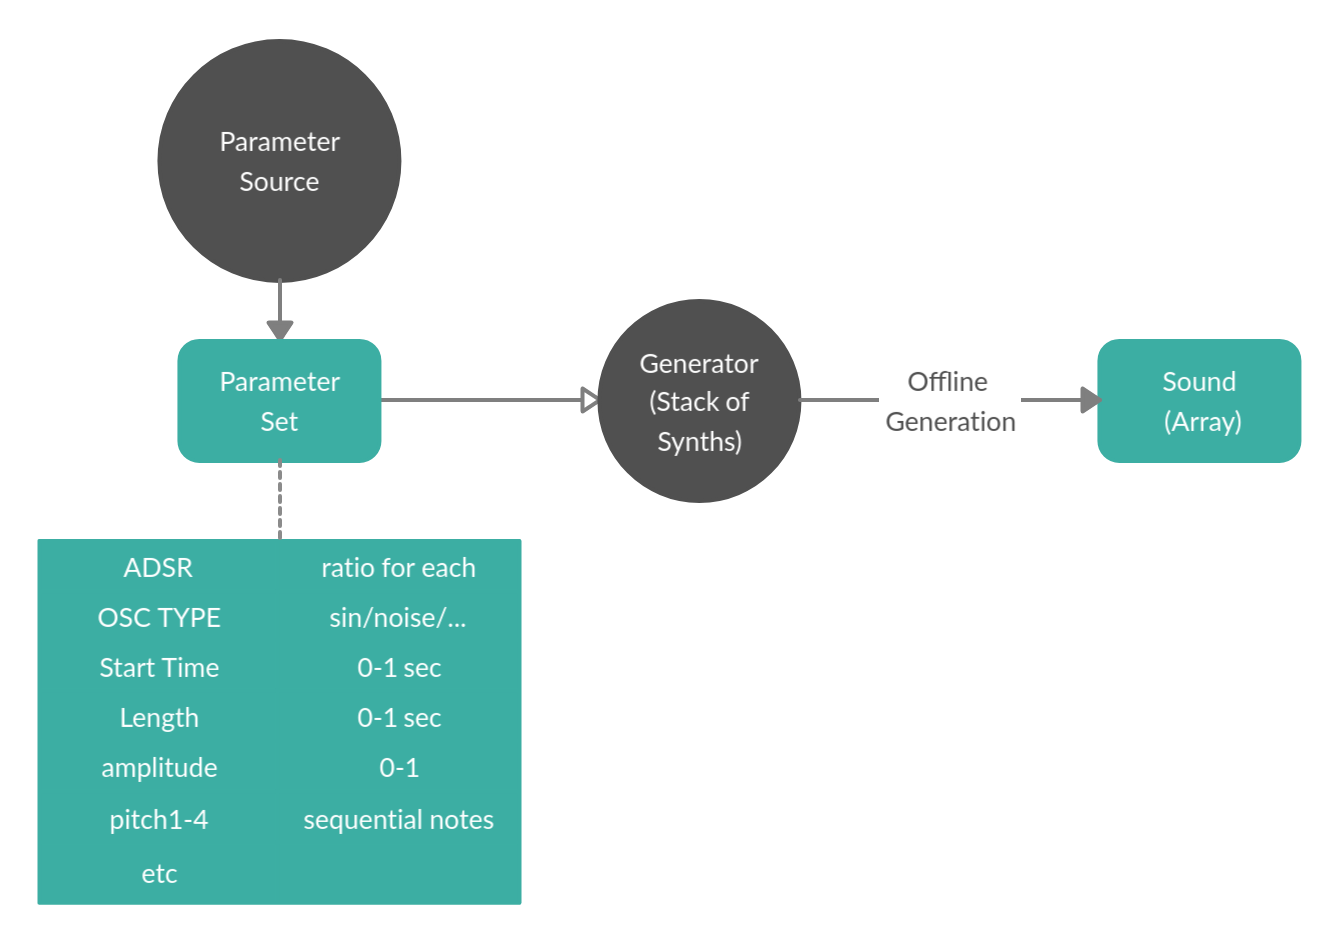
\includegraphics[width=0.9\textwidth]{images/SSS_gen.png}
% \caption{Generation Pipeline}
% \label{fig:SSS generator}
% \end{figure}

\subsection{The Generator}
We used the python based Pippi library for our generator implementation\footnote{https://github.com/luvsound/pippi}. This library uses a C back-end and focuses on fast offline generation. We define a Synth as the smallest unit of sound generation. A single Synth can be fairly expressive on its own, but we also allow a combination of Synths, which we call a Synth Stack. Each Synth takes in multiple parameters (parameter-set) and generates a sound. If the stack size is larger than 1, the combination of these individual parameter-sets is treated as the parameter-set for the stack. 

\subsection{The Ear}
The most challenging and important component of the project; the ear can be any method of evaluating a piece of audio. The most basic representation of a piece of digital audio is via list of numbers and a sampling-rate. For simplicity, we fix the sampling rate to 41,000 per second across all components of this project. An array representation of audio is the representation of the audio within the time domain. More commonly, the frequency domain is used for MIR tasks.
% \begin{figure}[H]
% \centering
% 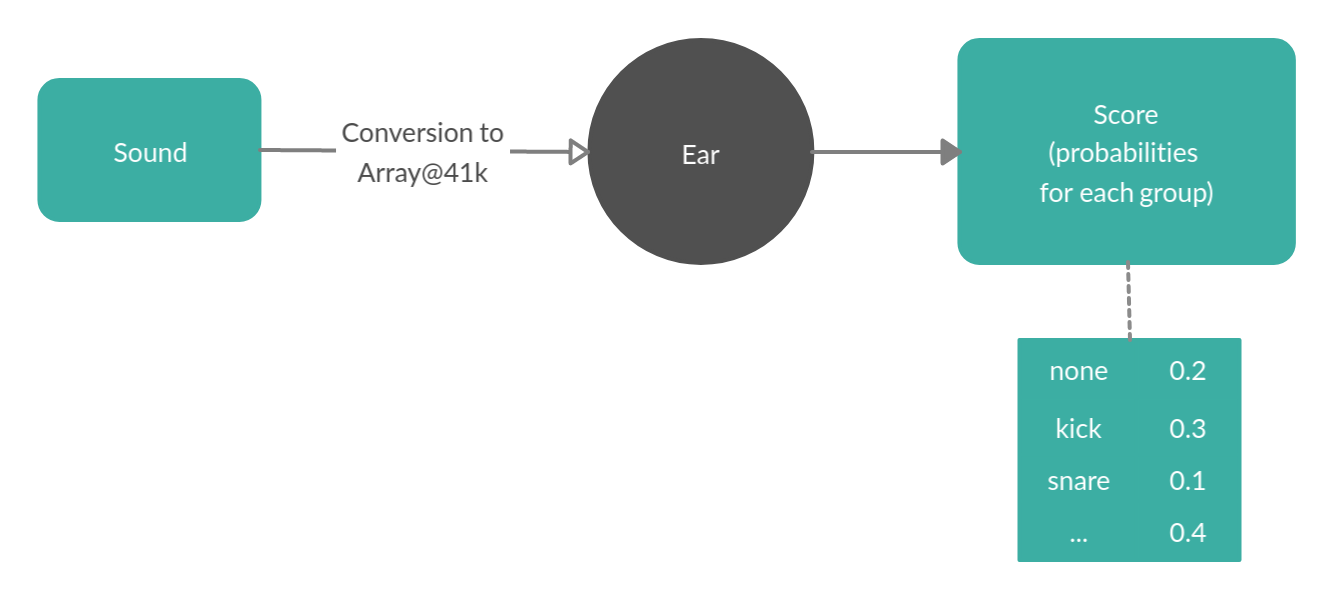
\includegraphics[width=\textwidth]{images/SSS_ear.png}
% \caption{Evaluation Using the Ear}
% \label{fig:SSS generator}
% \end{figure}

\begin{figure}[h!]
\centering
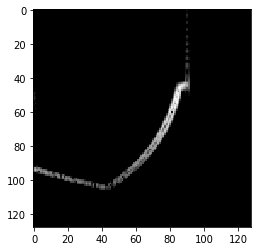
\includegraphics[width=0.5\textwidth]{images/specplot.png}
\caption{Mel-spectrum representation of a randomly generated sample}
\label{fig:SSS generator}
\end{figure}
All we require from the ear is to give us probabilities of an audio sample belonging to various sound (drum and none-drum) categories. It should be self-evident that these probabilities should sum up to 1.\\

We have implemented several methods of feature extraction thus far and successfully separated different drum categories in interesting ways, visualized in the "interactive\_separation\_graph.ipynb" notebook. A common pitfall of most feature extraction methods implemented is that they do not consider the temporal trends within the audio, making them highly susceptible to errors when evaluating audio that should not belong to any of the categories.\\
\todo[inline, color=green!40]{
Sanity Check: If a drum sample is reversed or chopped up, its likelihood of being labeled the same should change.}

There are two interconnected temporal trends to consider: 
\begin{itemize}
    \item Change in amplitude within each frequency bin. Harder to measure and utilize and possibly not as important for our purposes, considering the short length of our samples.
    \item Overall amplitude change within a sample. Closely linked to ADSR. 
\end{itemize}{}

Temporal trends are can be deduced from a spectrum representation of sound (at least visually by a human). A convolution net trained on our drum dataset led to an ear good enough to continue to the next stage of the project. The current model does an adequate job of rejecting junk data and semi-robustly rejects samples with inappropriate wave-shapes,\todo[color=red!40]{but leaves much room for improvements}.
\begin{figure}[H]
\centering
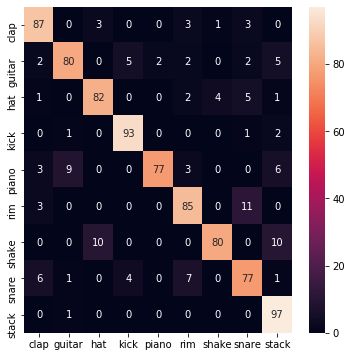
\includegraphics[width=0.8\linewidth]{images/cnn_ear.png}
\caption{CNN ear working well on a test set}
\label{fig:ok ear}
\end{figure}

\subsection{Generator+Ear}
Once we have a generator and an ear, we can quickly generate a large dataset where each data item is a random parameter-set, the ear score of the parameter-set and the corresponding rankings for each category. The rankings are derived from the probability scores. For example, the category with the highest probability will have the rank of 1, second highest would rank 2nd, and the lowest probability will have the rank of n (assuming n categories).\\
Important to highlight is that thus far we have only used 1 Synth to generate our sounds, but our generator has the capability to use larger Synth Stacks, and the pipelines are written with that possibility in mind.\\
\todo[inline]{A seen in Figure \ref{fig:rank portions}, there is a bias in random generation towards making higher ranking hats and kicks and lower ranking shakers, claps. Is this bias because of Synth structure or a problem with the ear?}
\begin{figure}[h!]
\centering
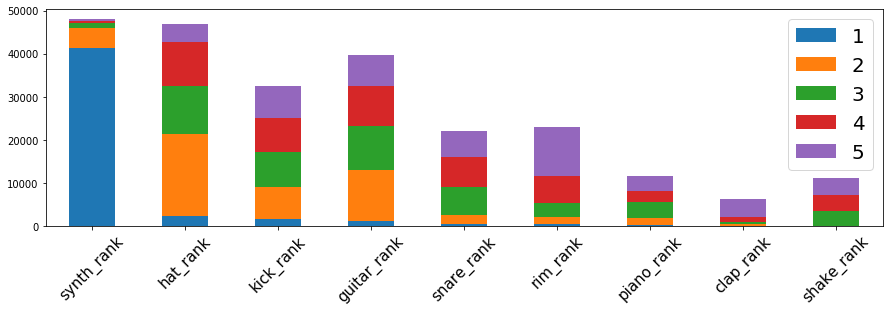
\includegraphics[width=1\linewidth]{images/random_ranks.png}
\caption{Figure showing proportions of categorical ranks for around 50,000 randomly generated sounds. Only showing ranks 1-5. About 90\% received the rank of 1 (blue portion of the bar) for the "synth" category, meaning that the ear correctly gave the highest probability to the sound being from a synth combination. We are interested in the small percentages of random generations that trick the ear due to coincidentally being similar to actual drums (i.e those who received a rank of 1) }
\todo[inline, color=green!30]{When looking for the best sounds of each category, could use ranks 2 and 3 etc. as well, however:
\unexpanded{\unexpanded{
\begin{itemize}
    \item We must figure out how to penalize their parameters
    \item The task requires even more confidence in ear,
    \item Generation is fast enough that we don't need to use ranks higher than 1. We have more than enough data if we don't want to deal with this task.
\end{itemize} 
}}} 


\label{fig:rank portions}
\end{figure}
\section{Novel Generations}
\subsection{Goal}
 Given a category, our aim is to use random generations to guide an algorithm towards novel generation of drums for that category.

\subsection{Guided Generation Attempts}

\subsubsection{Multivariate Normal}
Some success and extremely fast and scalable once the parameter space is calculated. Currently our parameters are array indices mapping to different values for Synth components. This makes the assumption that our discrete parameter space is normally distributed or differentiable in-appropriate and prone to errors. \todo[color=green!40]{provide example as proof. e.g: bimodal parameter}

\subsubsection{Evolutionary Search}
Implemented evolutionary search using DEAP \citep{DEAP_JMLR2012}. A parameter set is assumed to be an individual with each parameter being its genes. To measure an individuals fitness, we use the formula $fitness=score-rank$. As generations evolve, a Hall-of-Fame list with a fixed size tracks the best individuals to ever live in any given generation, updating itself after each batch of off-springs is evaluated.\\
To ensure diversity of the HOF individuals, the fitness score should also consider some measure of uniqueness. A weighted minkowski distance \footnote{https://docs.scipy.org/doc/scipy/reference/generated/scipy.spatial.distance.minkowski.html} between the genes of an offspring and the HOF individuals may be a good measurement.\todo[color=orange!40]{Medium Priority} \\
A generation of $N$ individuals are initialized(randomly or using already existing ranked parameters). To create the offspring generation, each generation goes through mutations and in-place gene crossovers. The new generation consists of the top 80\% of the offspring generation and 20\% new individuals to quicken gene diversity. If the new individuals are coming directly from previously measured high scoring parameter sets, we ensure that they cannot be directly added to HOF without going through mutations and crossovers first. 



\section{Priorities}
\subsection{Highest Priorities}
\subsubsection{Lit Review}
Extremely lacking at the moment. A few hours spent on the linguistics research was not very fruitful. Will revisit and further explore papers related to project magenta, WaveGans and adversarial audio generation in the upcoming days. \\
Also necessary is to search for related NIME papers to help with methodology improvements, paper motivation and guiding the writing process.  
\subsubsection{Ear improvements}
Great potential for improvements as well as great benefits for improvements make this the highest priority in terms of programming. A better ear means better generated sounds and more confidence in our measurements.
Relevant tasks:
\begin{itemize}
    \item Proper envelope detection
    \item LSTM ear
    \item Dealing with, and necessity of, a junk/noise class
\end{itemize}
\subsection{Medium Priorities}
\subsubsection{Search Improvements}
Search works but is highly dependent on the ear.\\ 
How well evo search work for each category? How to measure it "working"
\subsubsection{Using Stacks of size larger than 1}
Single stacks are powerful, but larger would be nice. 
\subsubsection{AutoEncoder Networks}
Implement variational auto-encoders for drum generation as an alternative to our method. 
\subsubsection{Generated Drums Survey}
Powered by 'diffrent music'. All we need is good generated drums.
\subsection{Low Priorities}
\subsubsection{SampleSwap}
Sign up
\subsubsection{Notebook Cleanups}
Cleanup notebooks, add them to the report
\bibliographystyle{plain}
\bibliography{references}
\end{document}
